\chapter{主播端的视频质量问题}
我们用开源的直播软件和Nginx服务器搭建了一个实验平台,测量在无线网络环境下,直播应用能否有效的应对复杂的网络状况。通过测量,我们发现开源软件的主播端在运行过程中会遇到传输质量不佳的问题,尤其是当网络带宽发生抖动时。为了验证目前商业级的直播平台是否也存在类似的问题,本章我们又进一步测量了一些流行的个人直播应用,如斗鱼和Twitch。大量的测量表明商业级的直播平台也存在一样的问题。之后我们通过跟踪开源直播应用的源码实现,找出了问题发生的原因。

\section{直播系统架构}
传统直播要求主播端必须具有良好的专用带宽,而且传统直播系统的端到端的时延很大,为数十秒量级。为了解决传统直播的上述问题,交互直播应运而生。个人交互直播与传统直播相比,有两大关键不同点:
\begin{itemize}
\item 个人移动设备作为主播端。传统的直播,比如ESPN,都是使用预留的专线连接将摄像机捕捉的高清原始视频传输到特定的源内容服务器,内容服务器将原始的视频转码切分为视频块,分发给每个观看的用户。个人交互直播的不同点在于,用户借助移动设备通过无线网络上传直播视频到源服务器,源服务器分发的过程和传统直播相同。无线网络环境下,移动主播经常会面临和别人一起竞争带宽的情况,同时由于主播的移动和移动环境中复杂的无线信号,个人交互直播可能遭受更多变的网络环境,面临的传输挑战更加严峻;
\item 移动直播要求主播和用户间的交互性。在传统的体育直播中,用户只是被动的观看直播,没有交互行为,也不需要得到反馈。交互直播由于存在主播和用户间的互动行为,端到端的时延至关重要,端到端的时延决定了主播和用户的交互体验。例如,如果用户给主播送礼物或者点赞,主播应尽快回复表示感谢,如果端到端的时延依然是传统直播的几十秒,用户的体验效果将会非常差。高交互性使得直播的延迟最多为几秒,远远小于传统直播的几十秒左右的端到端时延。
\end{itemize}

复杂多变的移动网络环境和高交互性的要求为优化交互直播的传输质量提出了很大的挑战。

\begin{figure}[h]% use float package if you want it here
  \centering
  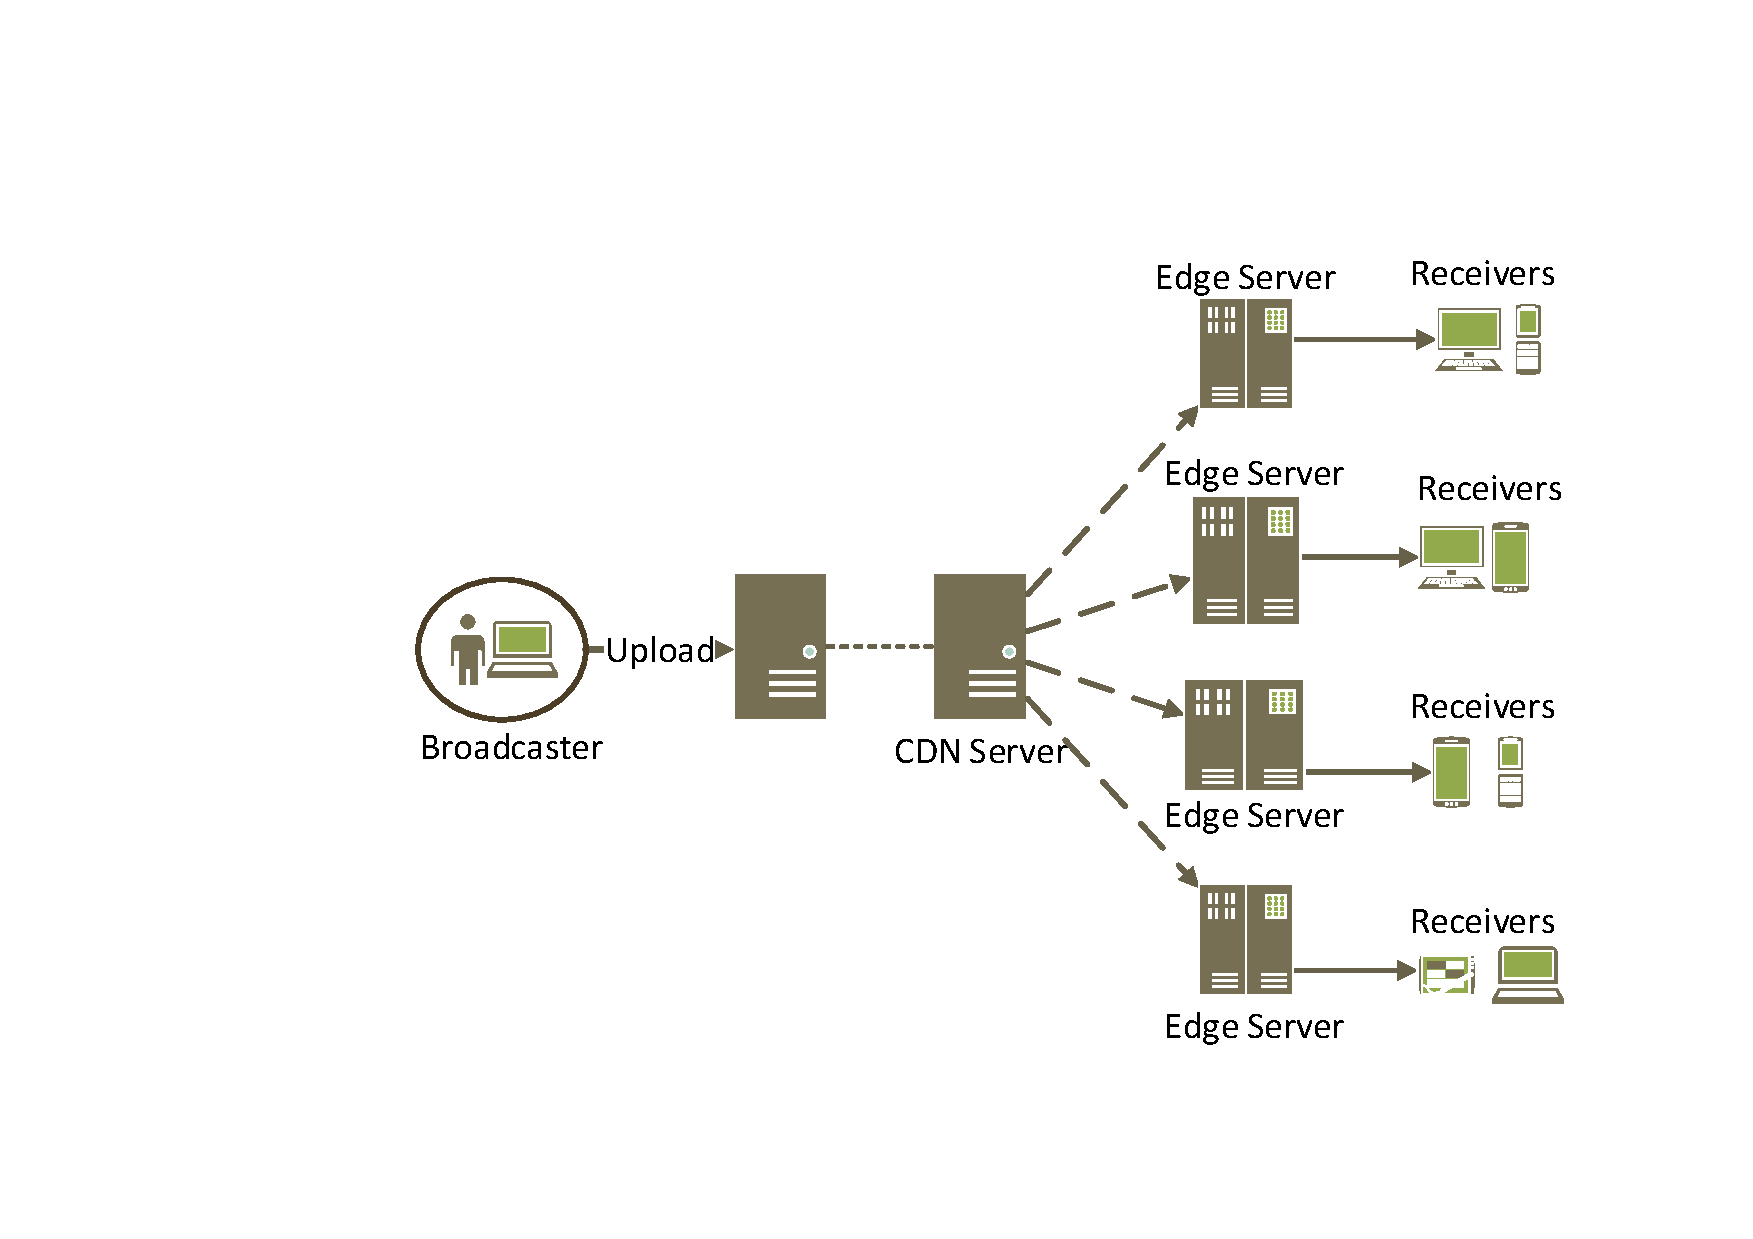
\includegraphics[width=0.8\textwidth]{architecture}
  \caption{交互直播系统架构}
  \label{fig:architecture}
\end{figure}

%可以阐述一下直播协议的事情

图~\ref{fig:architecture}给出了个人交互直播的常用架构。交互直播的过程一般可以分为三个部分,主播端到源服务器,源服务器到CDN边缘服务器,CDN边缘服务器到观众。开始直播时,一般主播端会通过特定的协议将直播的视频流上传到源服务器。主播端到源服务器端的协议多种多样,每个商业平台使用的协议都可能有所不同。多数的商业平台选择采用RTMP协议上传视频,少数的商业平台采用HTTP协议,也有部分平台使用自己定制的UDP协议去完成视频上传。源服务器在接收到主播端上传的直播视频流后,会首先将单一码率的视频流分别编码成多种码率。另外,如果通过CDN网络分发时使用的协议和主播端协议不一致,源服务器处会进行一定的转码操作。之后源服务器将编码后的视频流,选择合适的码率,转发至CDN分发网络;CDN网络将视频通过传统的overlay分发网络分发至CDN边缘服务器。最后,每个用户从最近的边缘服务器获取视频。CDN网络分发时使用的协议多数为HTTP协议,但也有少部分平台使用自己定制的UDP传输协议以减少端到端的时延。

\section{主播端性能测量}
\begin{figure}[h]% use float package if you want it here
  \centering
  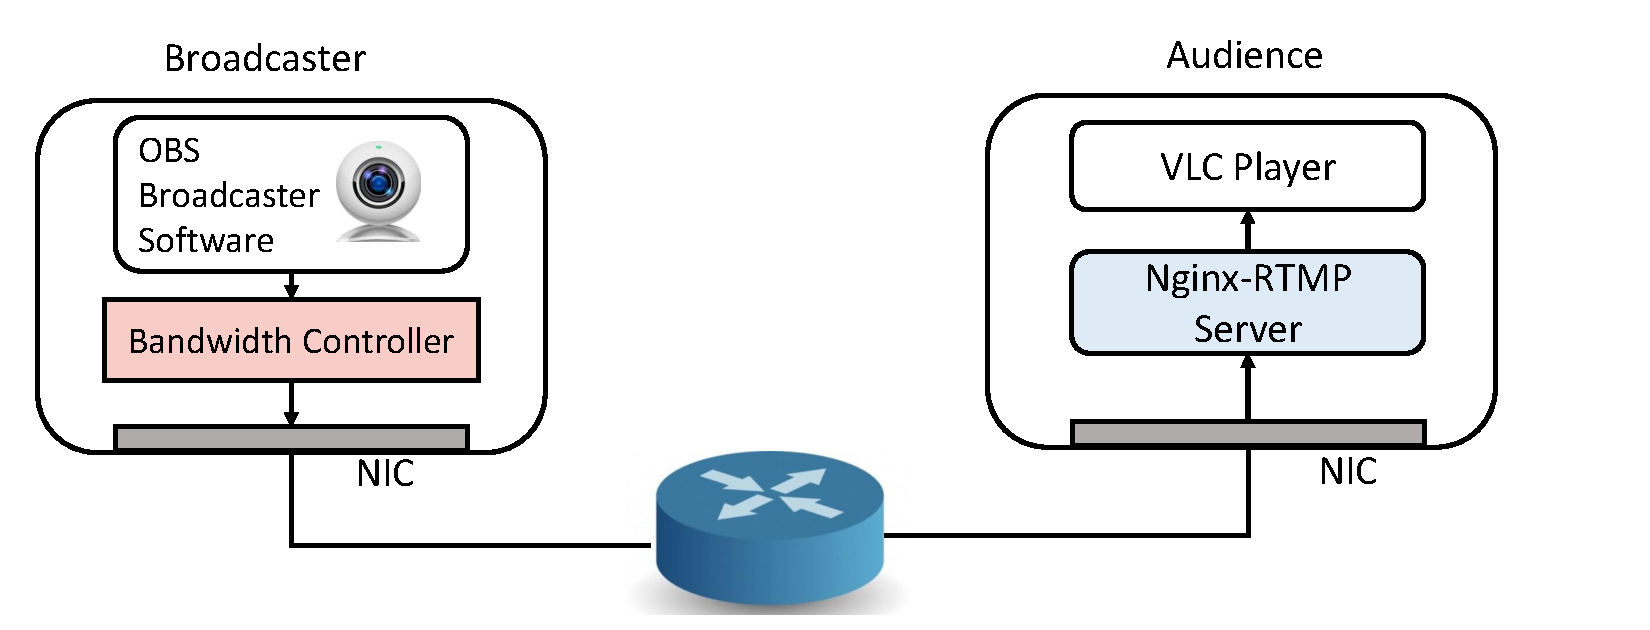
\includegraphics[width=0.8\textwidth]{setup}
  \caption{实验设置}
  \label{fig:setup}
\end{figure}

\textbf{实验设置} 我们搭建的直播传输架构如图~\ref{fig:setup}所示,包含两个主机和一个路由设备。 两端的设备(主播端和观众端)都配备有两个CPU,6G内存,设备的网卡带宽为100Mbps,他们通过中间的交换机连接在一起。主播端配备有摄像头,通过OBS软件将摄像头抓取的内容上传至直播服务器。OBS是一个开源的商业级直播软件~\cite{OBS},斗鱼和Twitch都将OBS作为推荐使用的直播软件。另外,OBS主要是使用RTMP协议来完成视频的上传。我们在主播端实现了一个带宽控制的模块,能够实时模拟无线环境的网络带宽变化。带宽控制模块在Linux系统下用Linux系统自带的tc模块实现,在Windows系统下则用dummynet~\cite{dummynet}来实现。在观众端,我们使用nginx的nginx-rtmp模块搭建了一个RTMP服务器,用来接收主播端上传的视频。另外,我们用VLC播放器去播放RTMP服务器接收到的直播视频流。

\subsection{案例分析:带宽抖动导致传输质量差}
为了尽量真实地模拟无线网络环境,我们使用真实的数据记录去控制实验的带宽变化。当用户通过移动设备浏览亚马逊网站时,每隔5秒给服务器发送探测到的实时带宽信息,我们以这种方式获取数据记录。我们将整个直播过程切分为多个5秒的时间段,将每个时间段内发送的所有数据报文聚合在一起,然后计算每个时间段内的总数据量,之后根据带宽的实际数值去控制主播端的网络带宽。我们选取其中260秒的记录作为具体案例,这一段数据的平均带宽在3300kbps以上。 实验一开始我们把直播的码率设为3300kbps,低于平均码率,这是为了防止整个过程码率始终低于平均值,无法判断出直播平台应对网络抖动的能力。启动OBS,上传摄像头抓取到的视频;与此同时,在观众端启用tcpdump去实时抓取报文。整个过程实时的吞吐量结果如图~\ref{fig:case_study}所示,为了更清晰的展示实验结果,我们把数据记录分为两个部分,0-140秒以及120-260秒。

\begin{figure}[h]
  \centering%
  \begin{subfigure}{0.49\textwidth}
    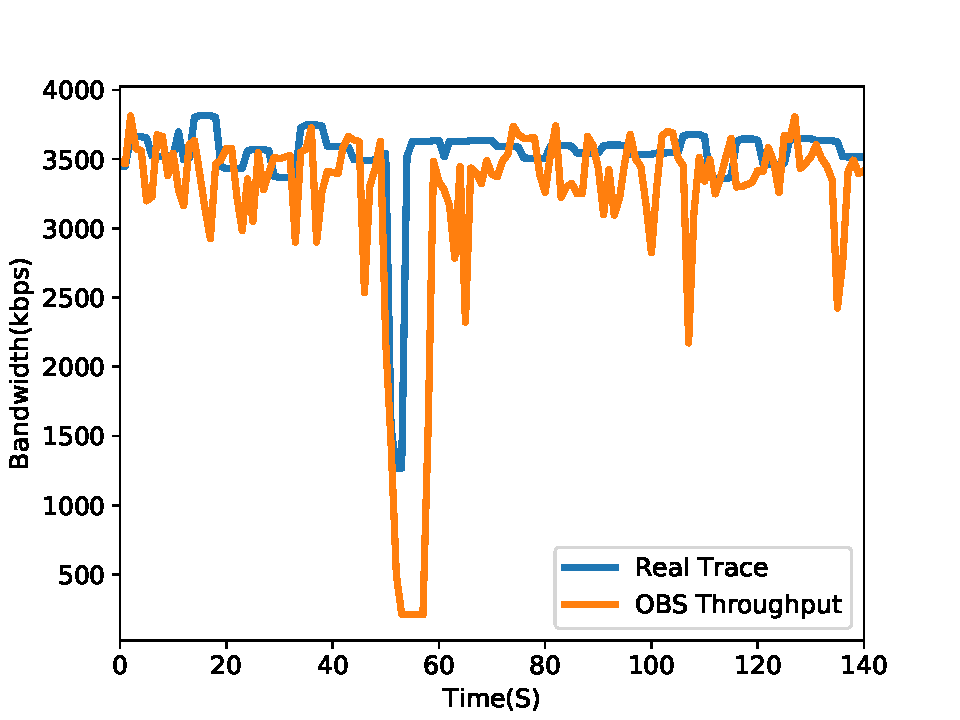
\includegraphics[width=\textwidth]{case_study_throughput_a}
    \caption{0-140s的吞吐量}
    \label{fig:case_study_a}
  \end{subfigure}%
  \hfill
  \begin{subfigure}{0.49\textwidth}
    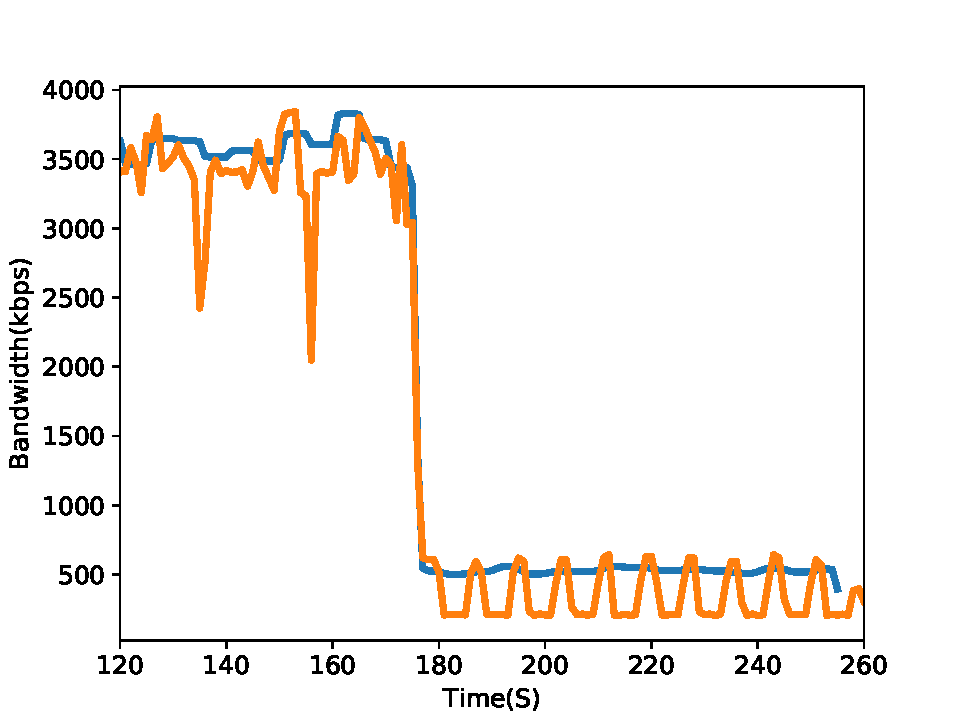
\includegraphics[width=\textwidth]{case_study_throughput_b}
    \caption{120-260s的吞吐量}
    \label{fig:case_study_b}
  \end{subfigure}
  \vspace{0.1in}
  \caption{无线网络环境下直播应用的吞吐量}
  \label{fig:case_study}
\end{figure}

仔细观察上述实验图,我们可以得出以下两个结论。(1)从图~\ref{fig:case_study_a}我们可以看出,大部分时间里,主播端的实际带宽一直紧紧跟随控制带宽发生变化。然而,在50秒附近,带宽大幅度衰减,低于初始的码率,维持在1500kbps左右,这种情况维持了2秒钟。此时,真实的数据吞吐量基本降为0,这一现象维持了8秒钟,从50秒到58秒。这是一种不正常的现象,2秒的网络抖动导致了直播流8秒的吞吐量下降。(2)从图~\ref{fig:case_study_b}可以看出码率固定的策略并不能有效的应对长时间的带宽变化。0-180秒期间带宽始终是充足的,高于实时的码率3300kbps,但是180秒之后带宽急剧变化,下降到500kbps左右,这个过程持续了80秒的时间。在这期间主播端显示,发生了大量的丢帧。在网络很差的环境下,OBS主播端依然维持在默认的码率值,但实时带宽远远小于码率值,网络无法将产生的视频流推送出去,这个策略显然不能达到很好的效果。

\subsection{带宽抖动的普遍性}
\begin{figure}[h]
  \centering%
  \begin{subfigure}{0.49\textwidth}
    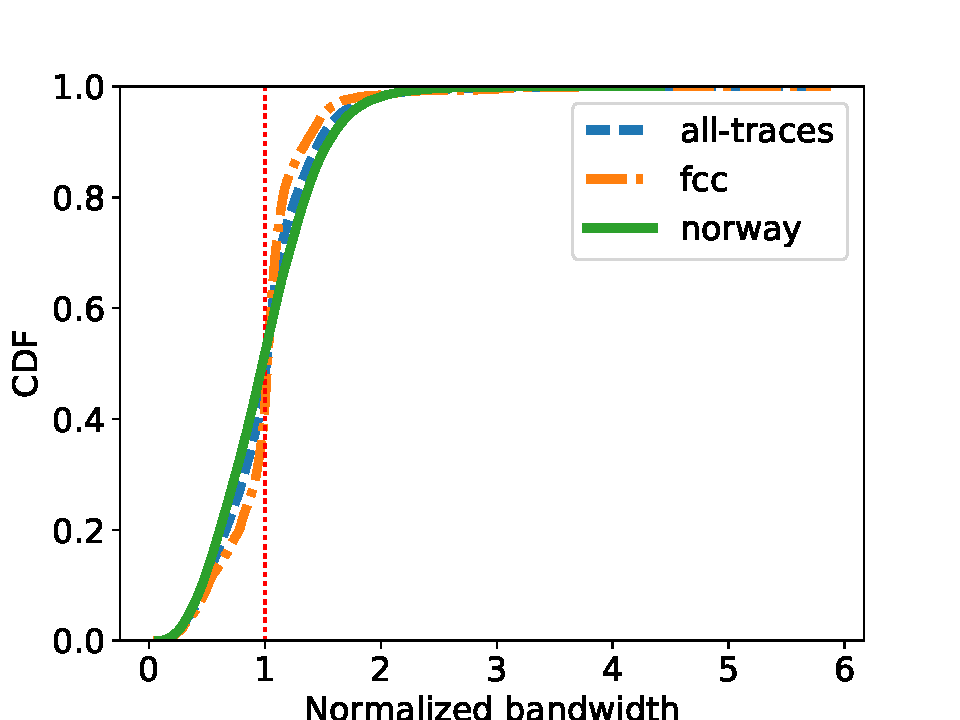
\includegraphics[width=\textwidth]{trace}
    \caption{归一化带宽累计分布函数}
    \label{fig:trace}
  \end{subfigure}%
  \hfill
  \begin{subfigure}{0.49\textwidth}
    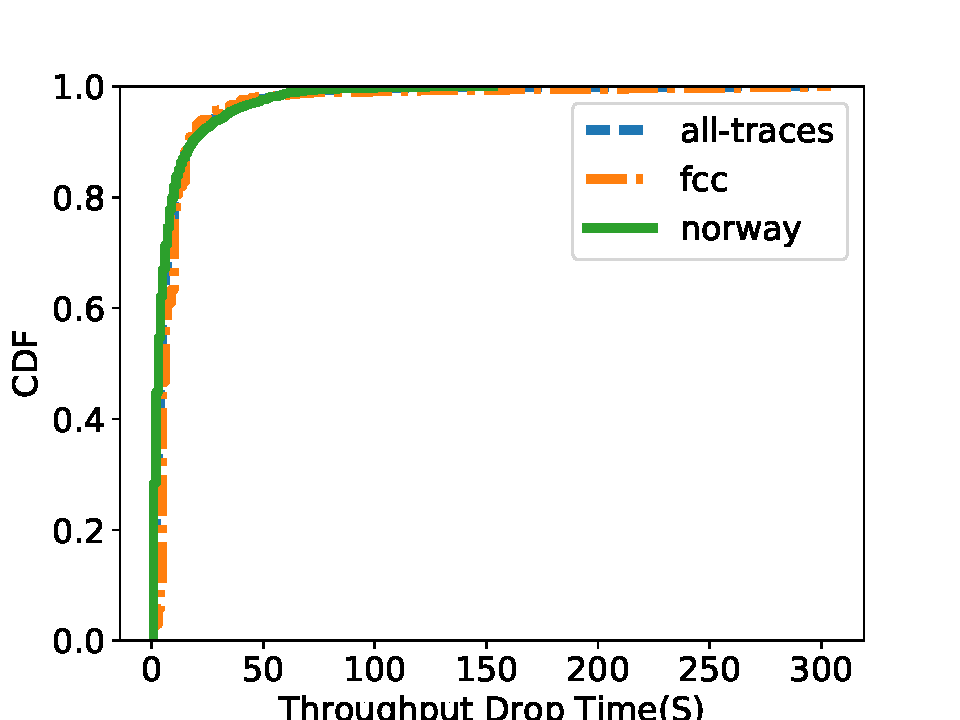
\includegraphics[width=\textwidth]{trace-down}
    \caption{带宽抖动时长分布}
    \label{fig:trace_down}
  \end{subfigure}
  \vspace{0.1in}
  \caption{无线网络环境的带宽分布}
  \label{fig:trace_distribution}
\end{figure}

为了评估无线网络环境下带宽抖动发生的频率,我们将两个真实的大规模公开数据集组合起来,以便数据分析。两个公开的数据集分别是Wifi网络环境下的FCC数据集~\cite{FCC}和移动网络环境下的HSDPA数据集~\cite{riiser2013commute},其中每个数据记录的持续时长为320秒,两个数据集的总共持续时间为30多个小时。针对每一条数据记录,我们把平均带宽作为单位数,去归一化每个数据记录的所有数据点,总的cdf图如图~\ref{fig:trace}所示。有50\%左右的时间,记录的数值小于平均带宽,这意味着对于一个10秒的带宽记录来说,有5秒的时间,实时带宽会低于平均值。20\%的情况下记录的数值只有平均值的一半。总的CDF分布图表明在真实网络世界中,带宽波动出现的很频繁。

为了进一步说明每次带宽抖动持续的时间,我们画了一张带宽抖动时长分布的CDF图~\ref{fig:trace_down}。带宽抖动时长是通过计算带宽在平均值以下的持续时间。大约20\%的网络抖动其持续时长多于10秒,有些甚至持续数百秒。另外,我们在上面的两张图中还分别画出了FCC数据集和HSDPA数据集的带宽分布和抖动时间分布,两个数据集单独的分布和整体分布相同,差别不大。

\subsection{商业平台验证}

\begin{figure*}[htb]
  \centering%
  \begin{subfigure}[b]{\textwidth}
    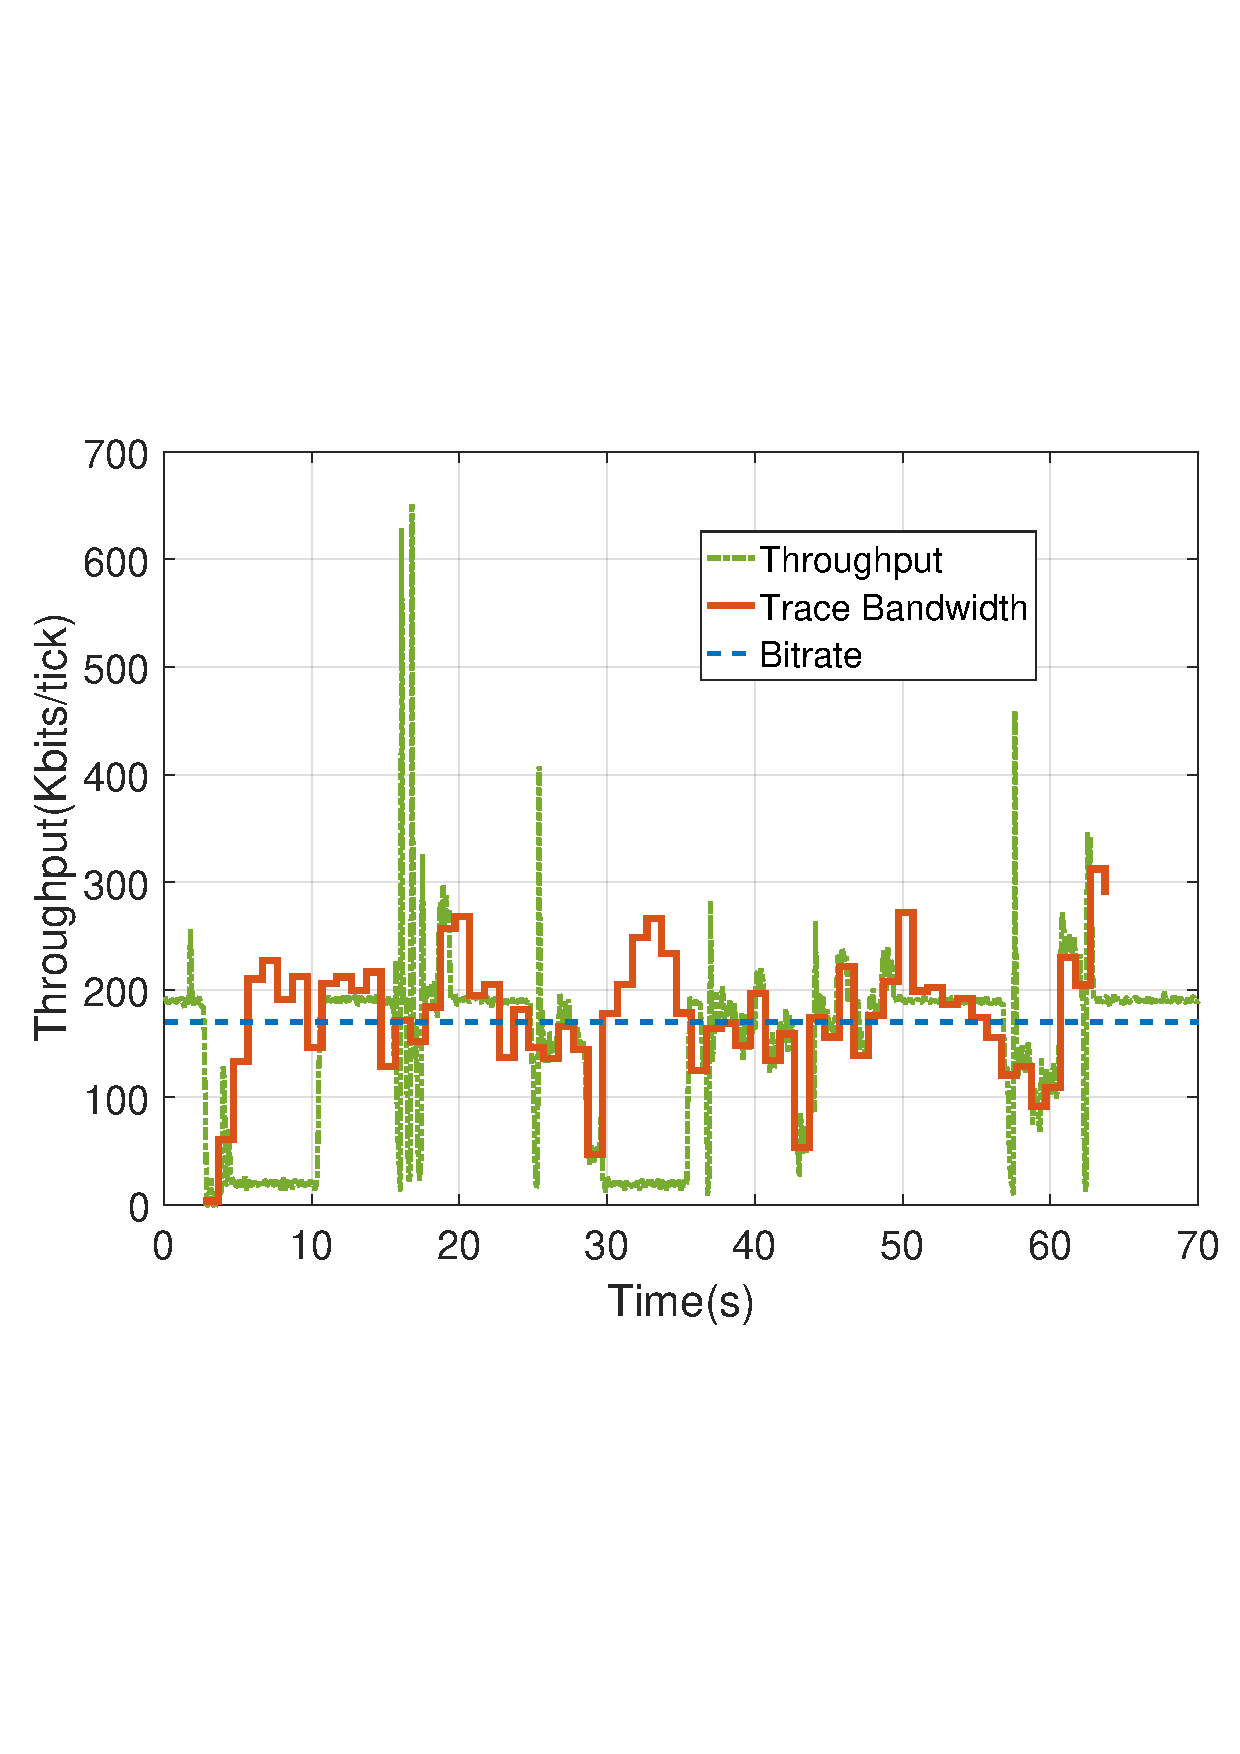
\includegraphics[width=0.46\textwidth]{obs_douyu}
    \hfill
    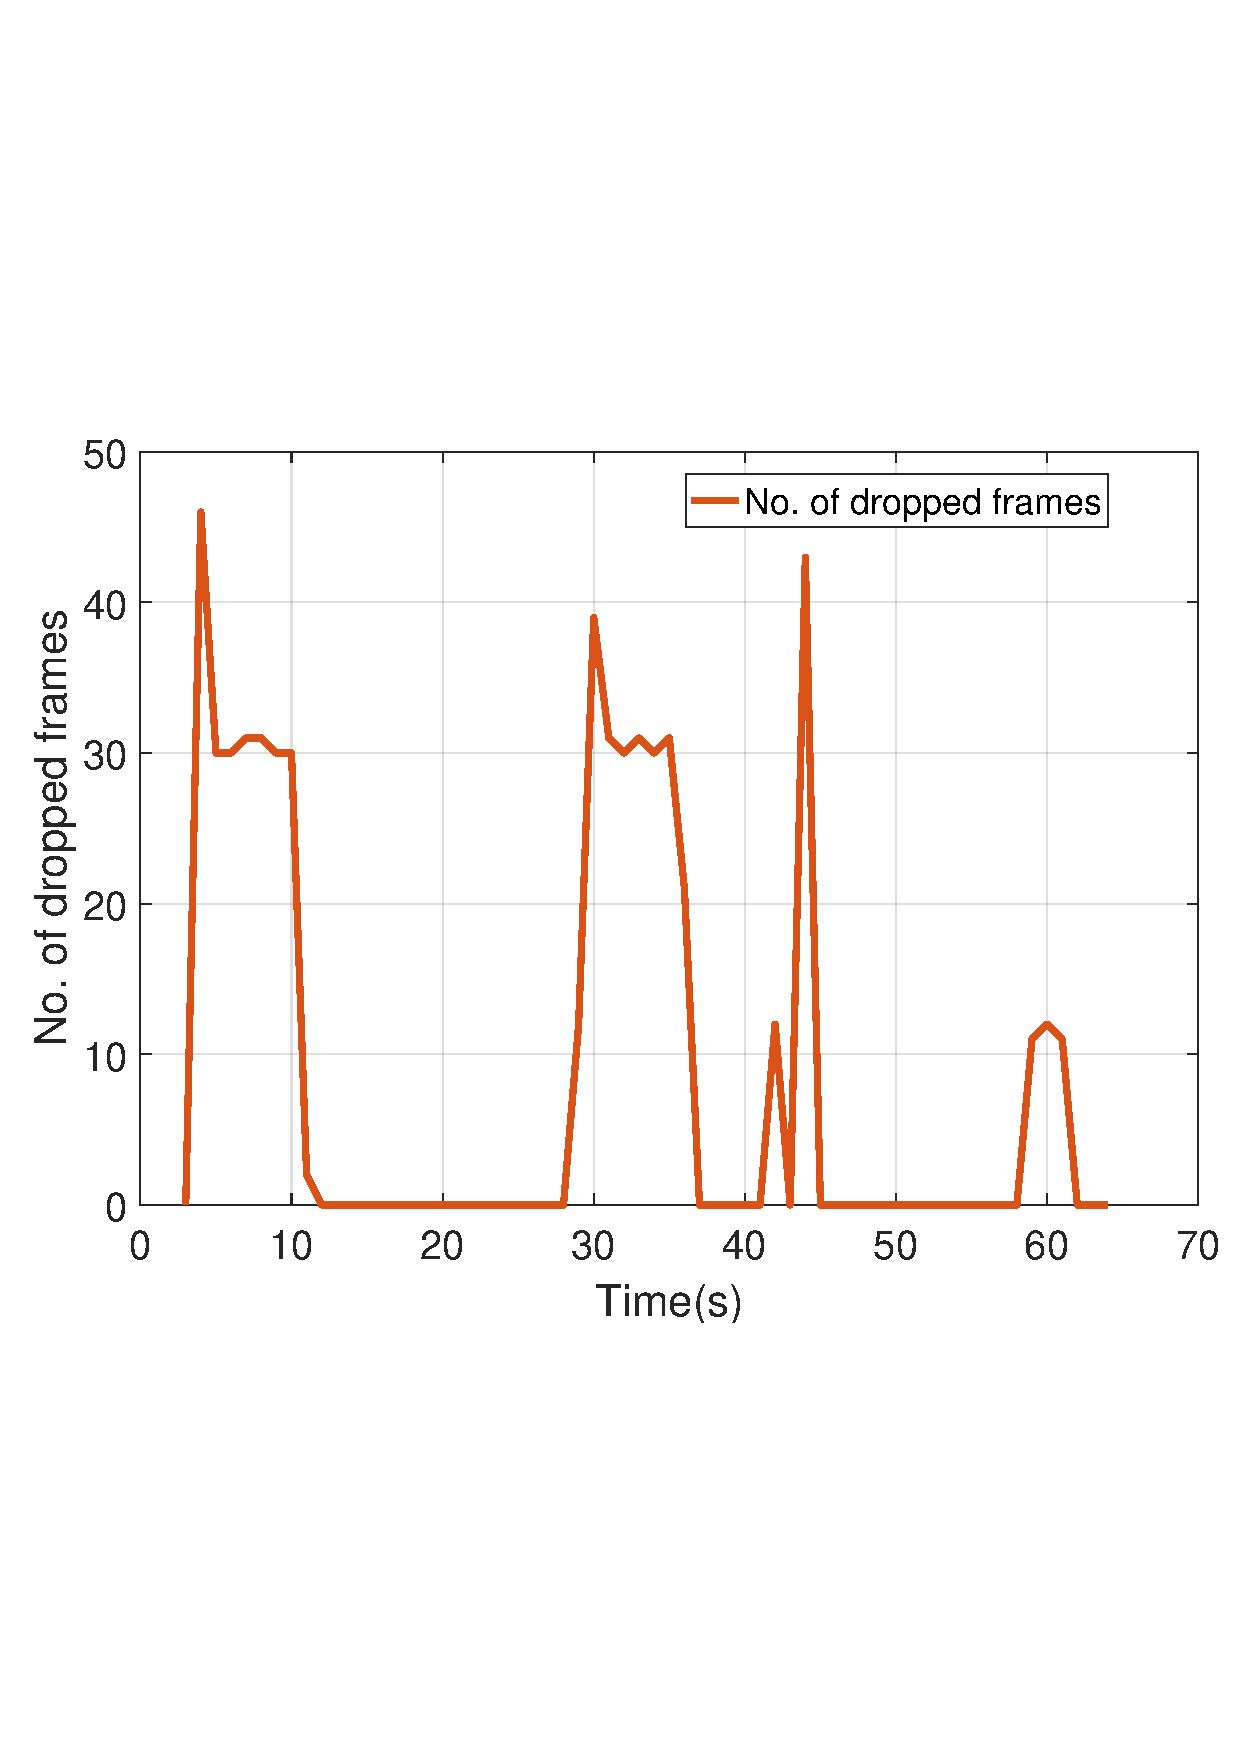
\includegraphics[width=0.46\textwidth]{obs_douyu_drop}
    \caption{OBS推流至斗鱼服务器的吞吐量和丢帧}
    \label{fig:obs_douyu}
  \end{subfigure}
  \vfill
  \vspace{0.2in}
  \begin{subfigure}[b]{\textwidth}
    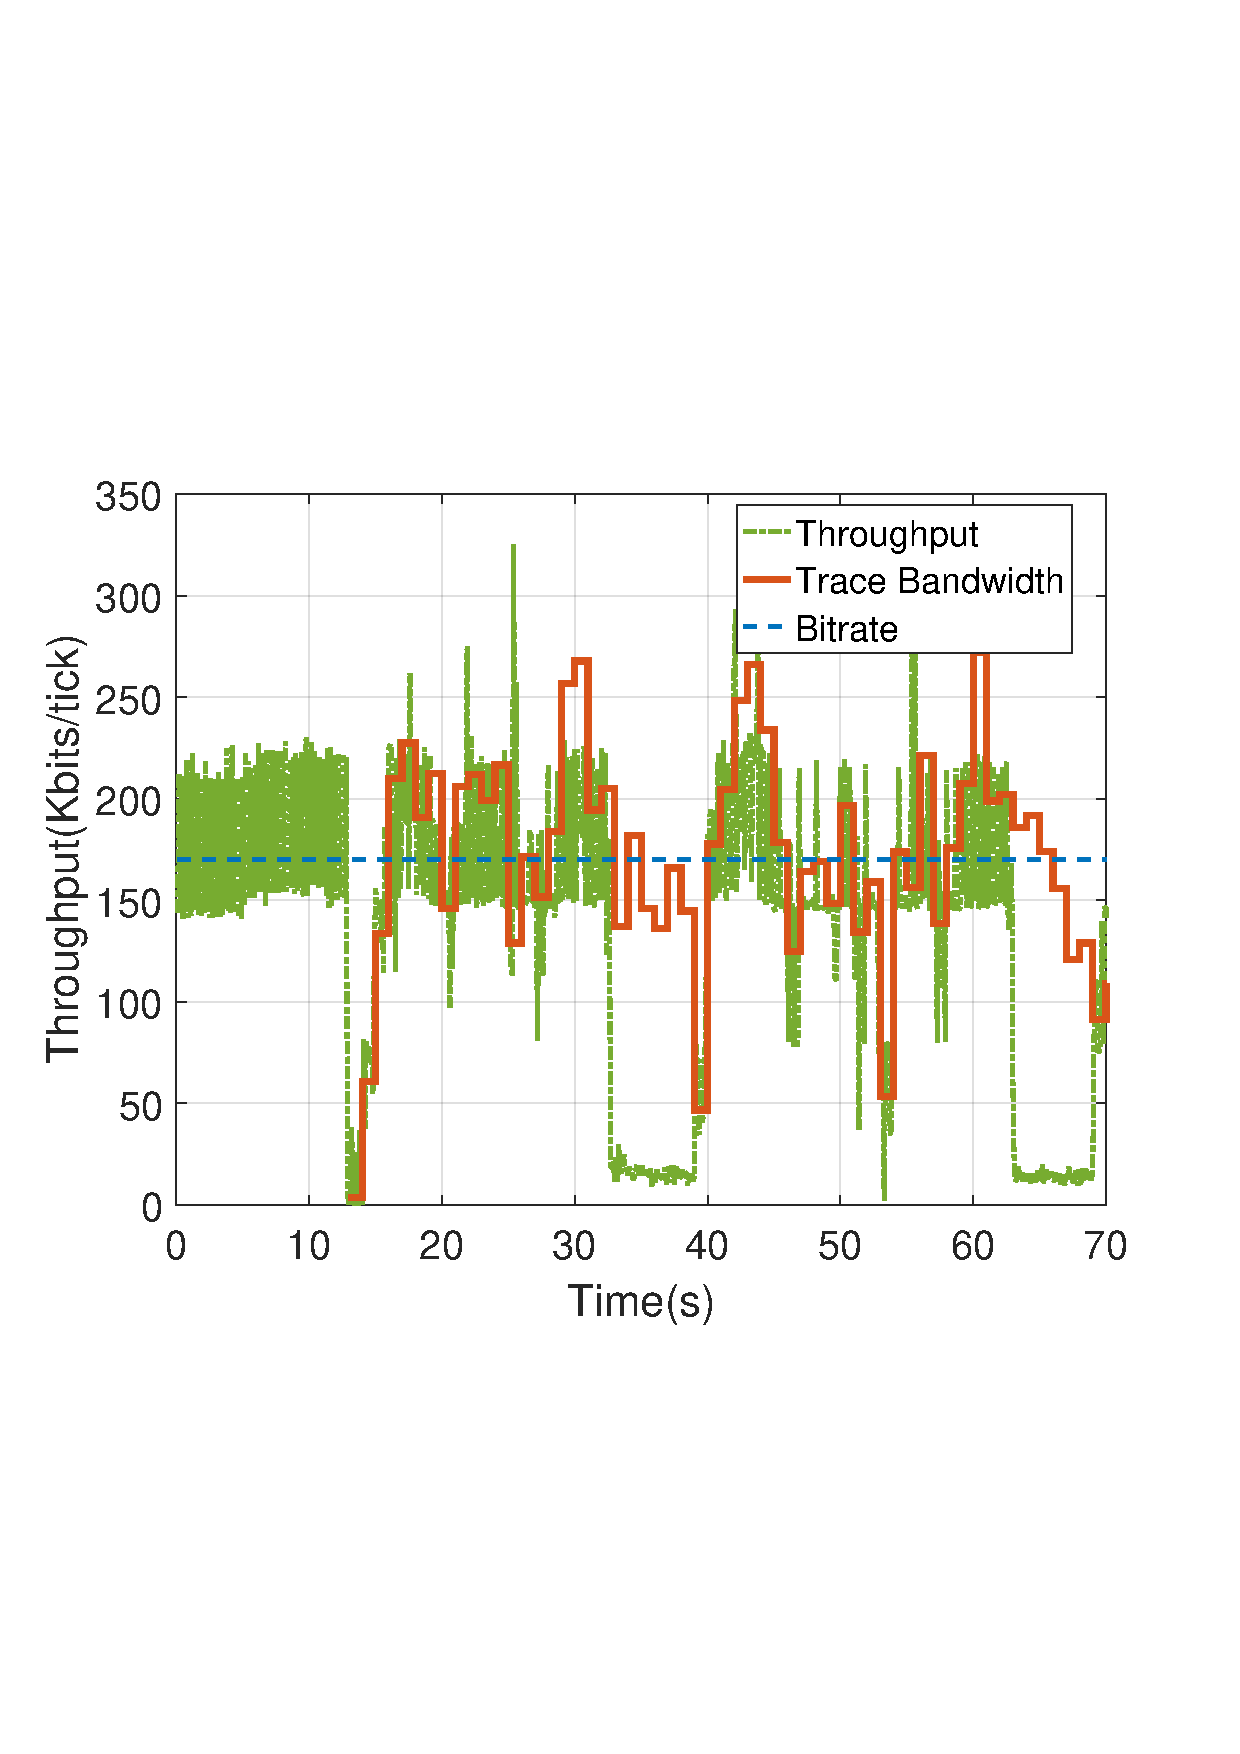
\includegraphics[width=0.46\textwidth]{douyu}
    \hfill
    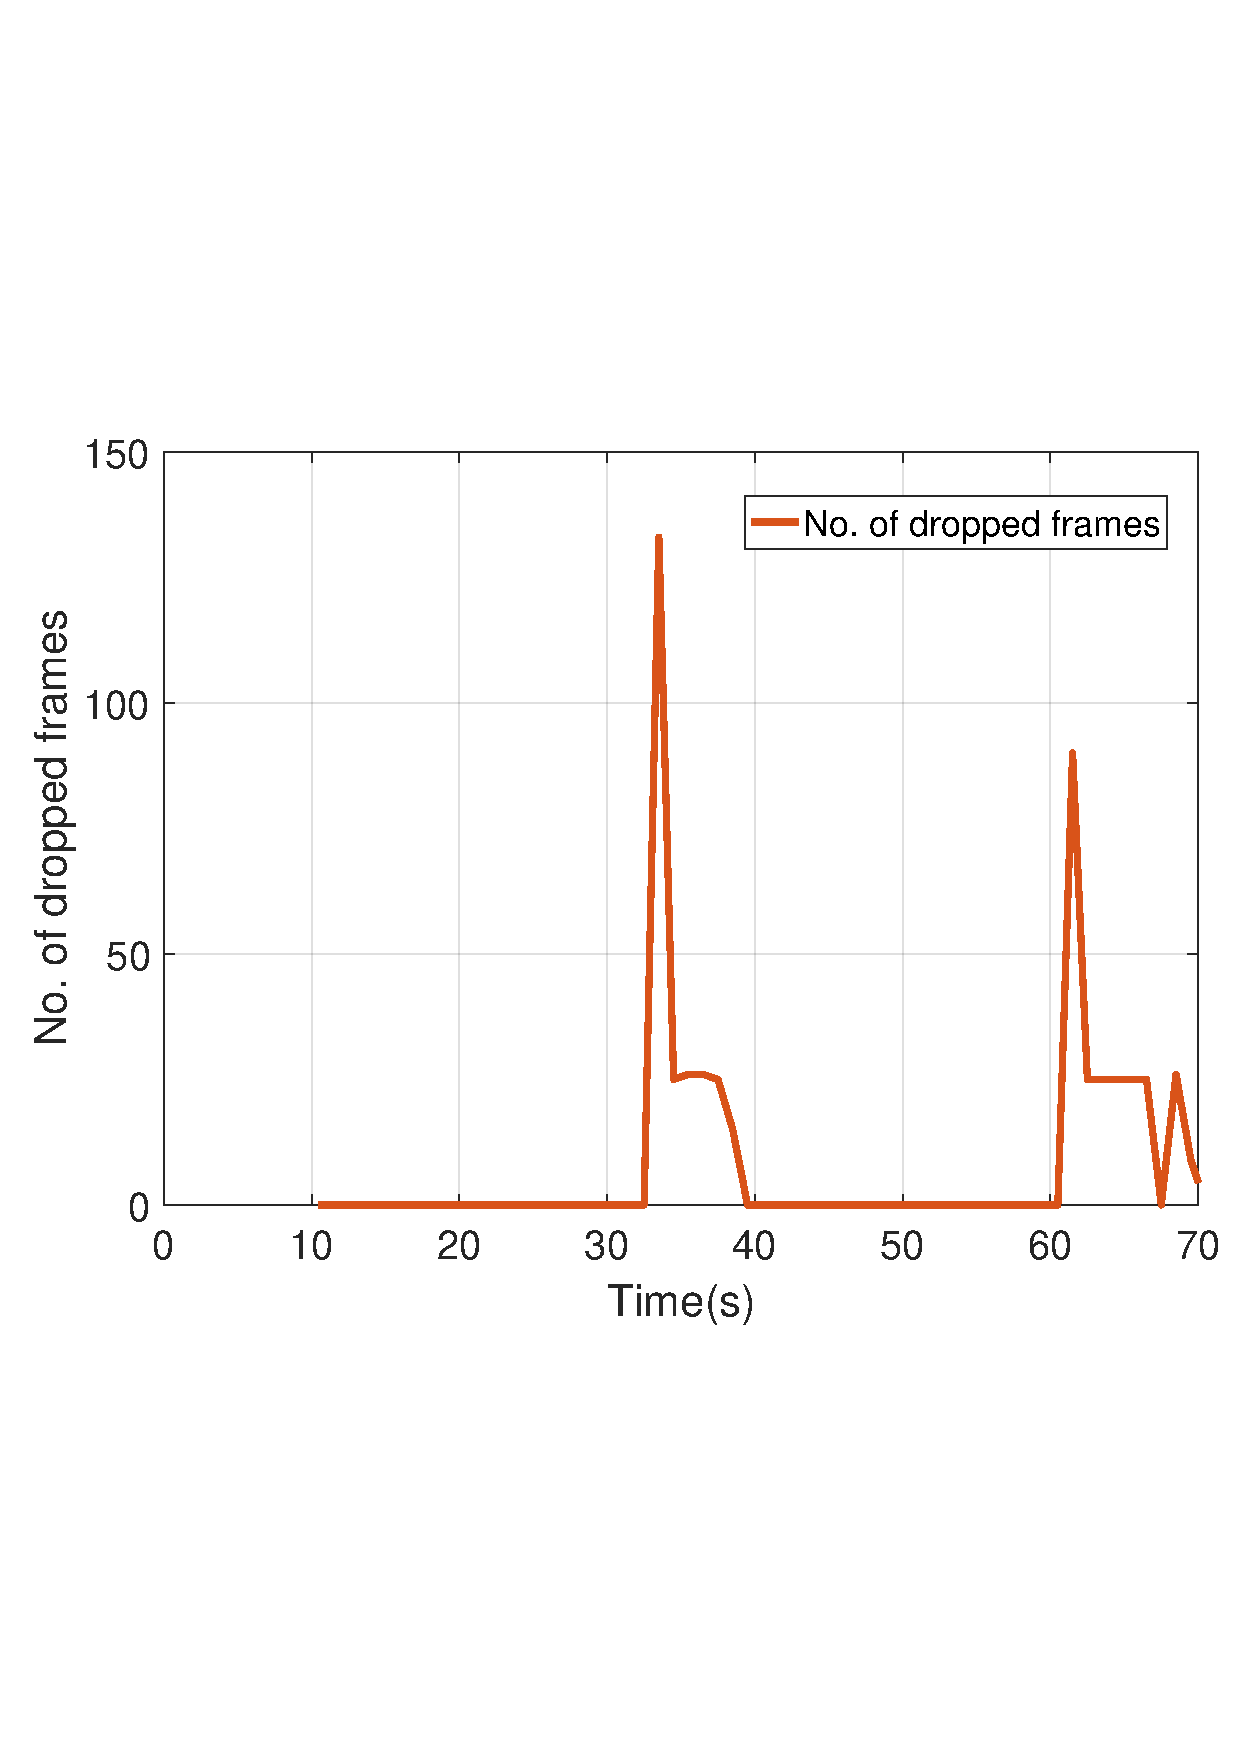
\includegraphics[width=0.46\textwidth]{douyu_drop}
    \caption{斗鱼主播工具推流至斗鱼服务器的吞吐量和丢帧}
    \label{fig:douyu}
  \end{subfigure}
  \vfill
  \vspace{0.2in}
  \begin{subfigure}[b]{\textwidth}
    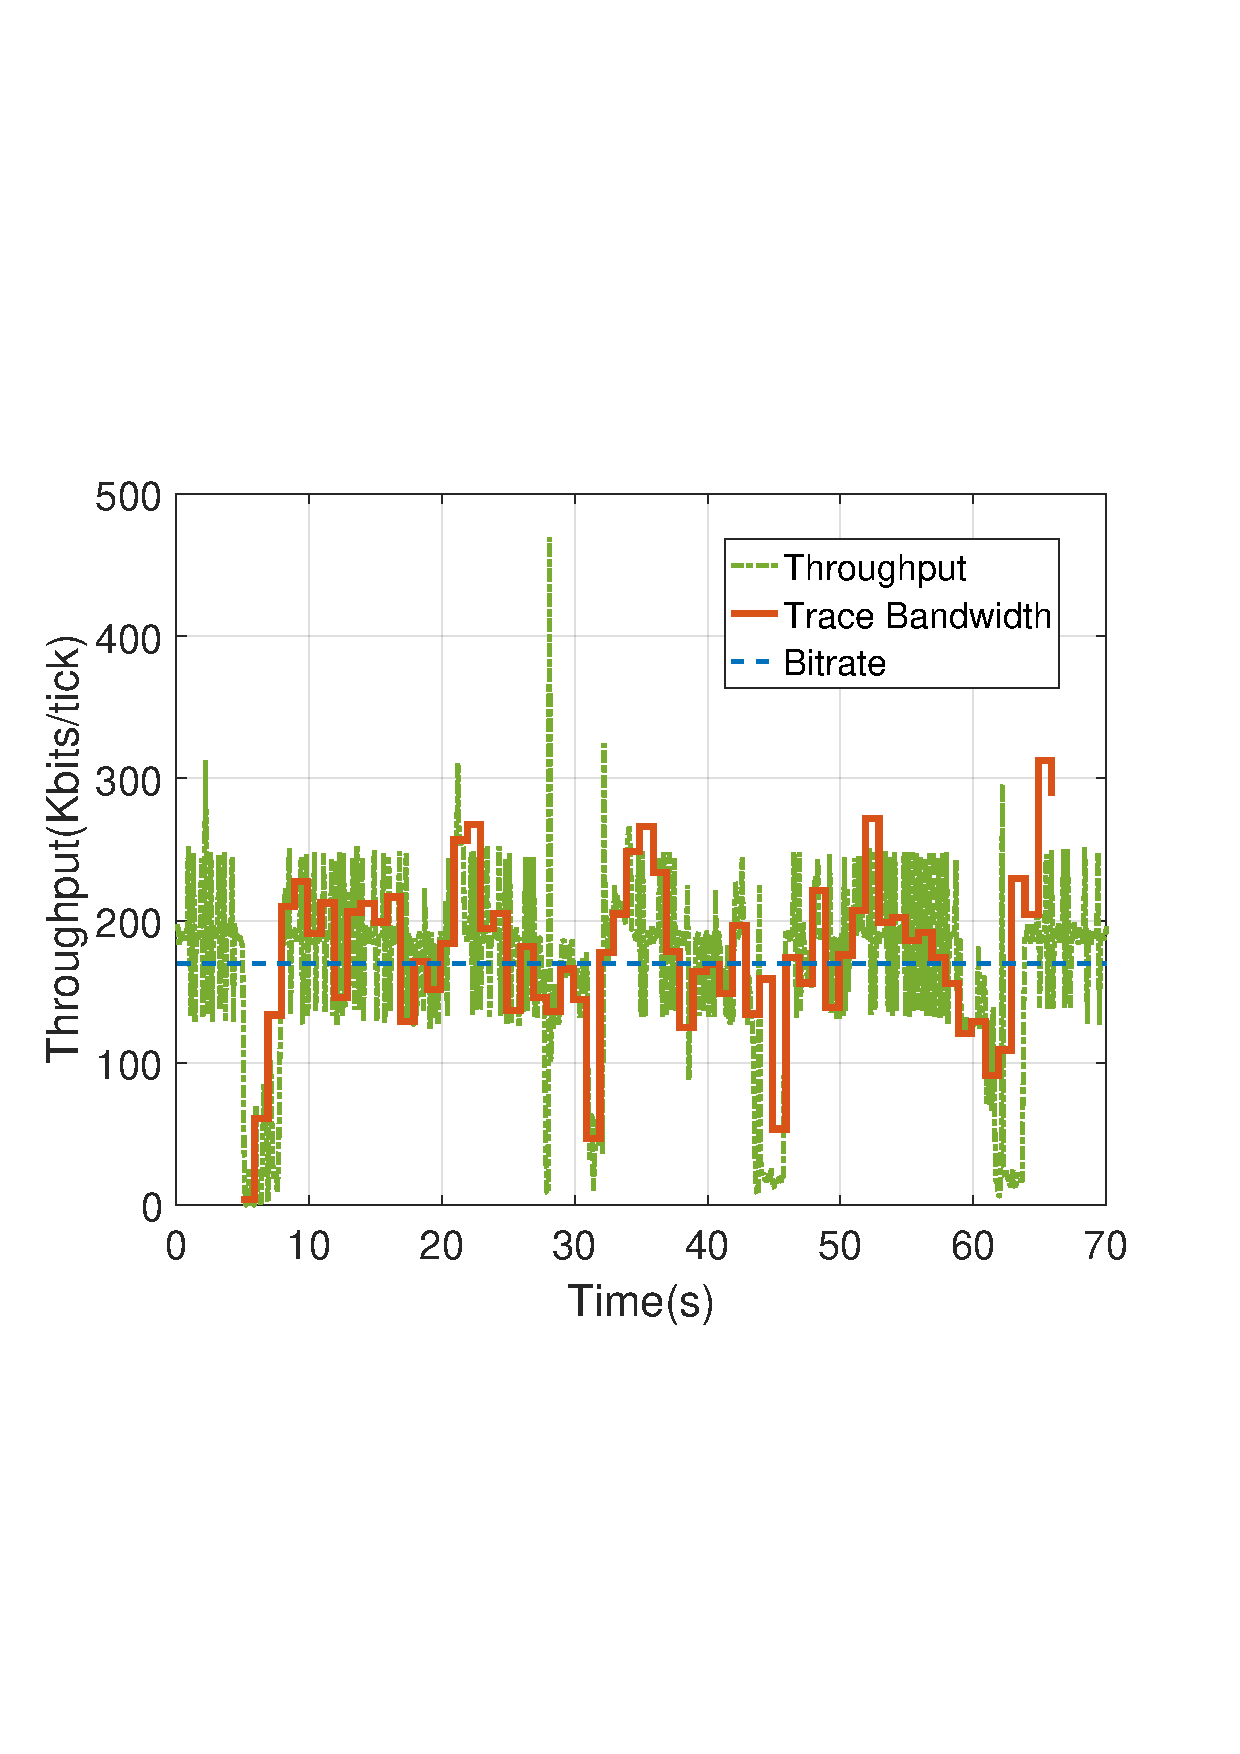
\includegraphics[width=0.46\textwidth]{obs_twitch}
    \hfill
    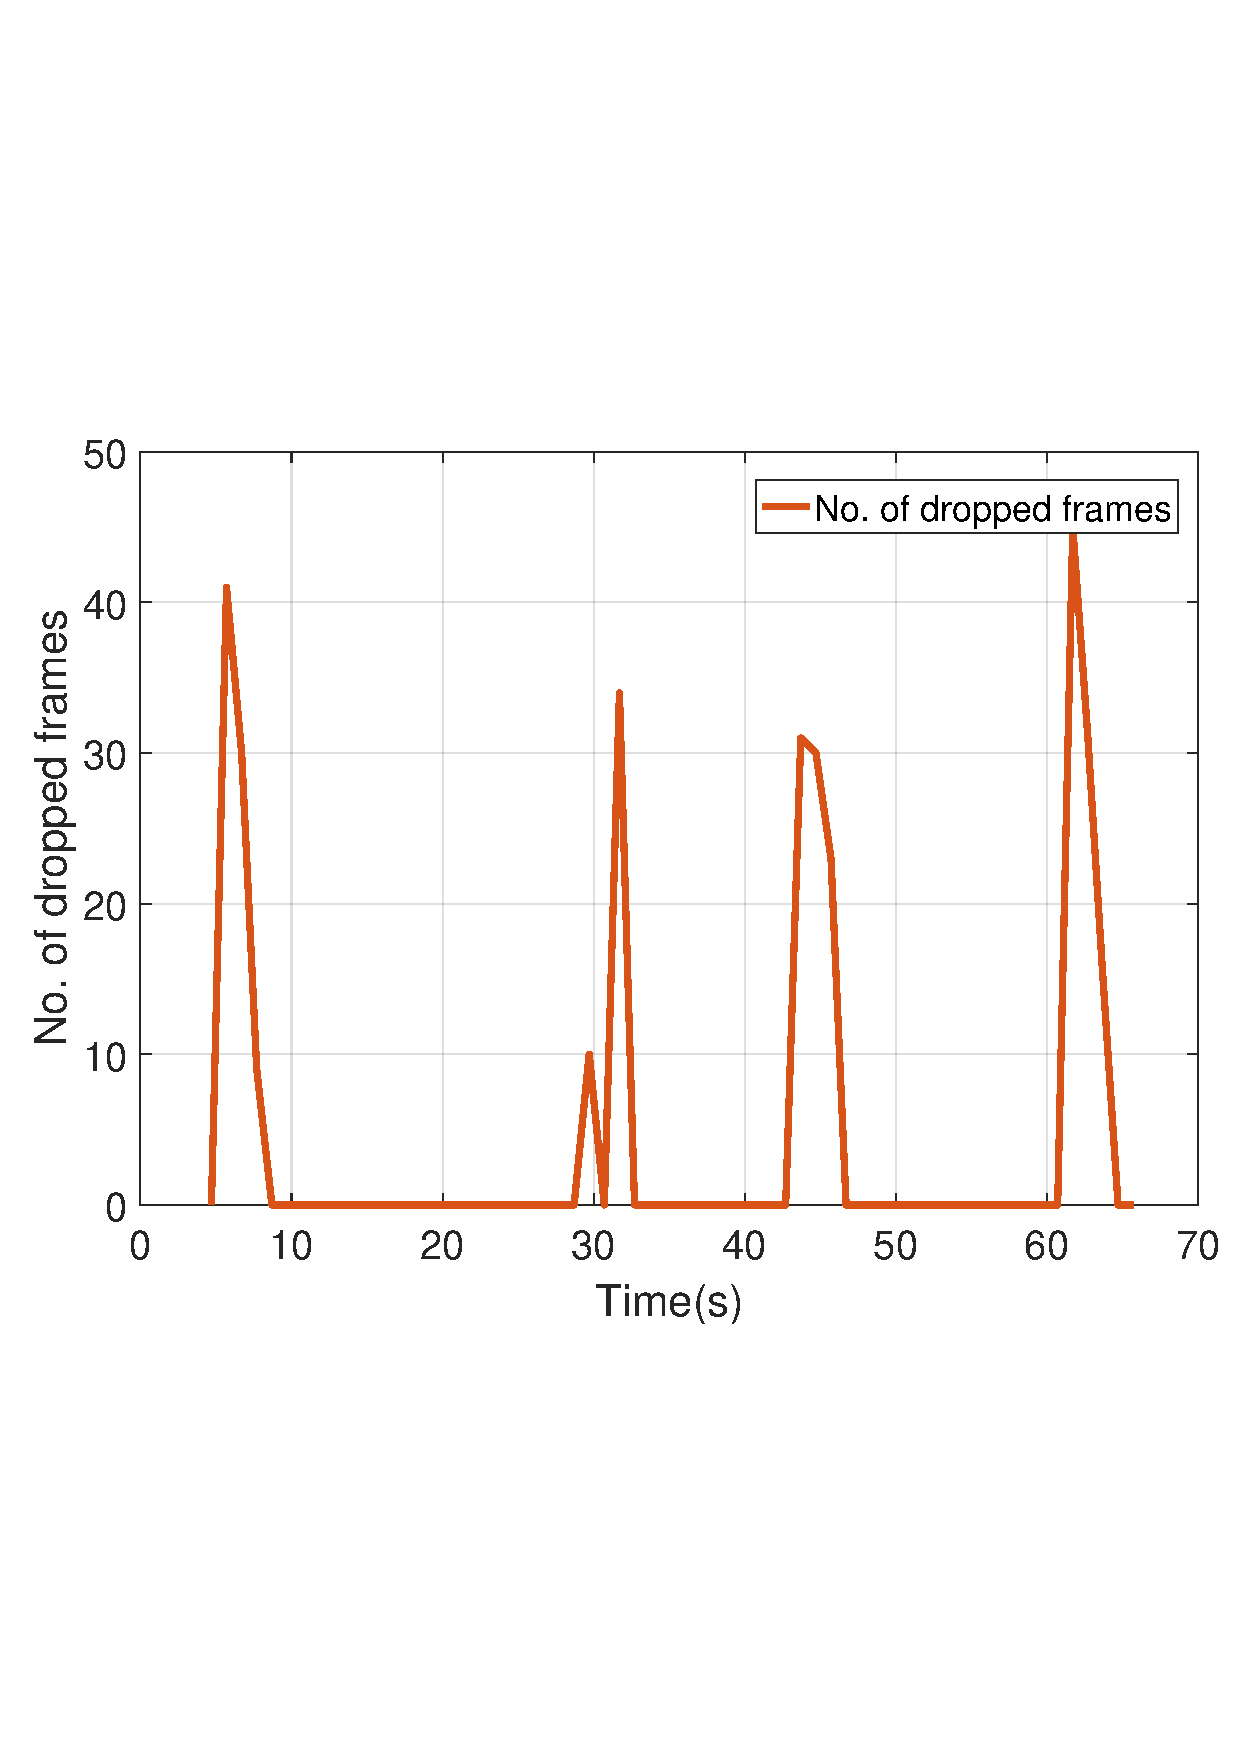
\includegraphics[width=0.46\textwidth]{obs_twitch_drop}
    \caption{OBS推流至Twitch服务器的吞吐量和丢帧}
    \label{fig:twitch}
  \end{subfigure}
  \caption{商业平台验证实验}
  \label{fig:commerical_application}
\end{figure*}


经过对真实网络环境的分析,我们发现在无线网络状况下,带宽抖动发生的次数较为频繁,且每次带宽抖动都会持续一定的时长。通过对开源直播软件OBS的测量实验发现,带宽抖动情况下OBS会遇到视频质量下降的问题。为了验证流行的商业平台上是否存在相同的问题,我们选择了几个交互直播的商业平台去重复上述的实验。分别是OBS作为主播端推流到斗鱼服务器,斗鱼主播工具推流到斗鱼源服务器,OBS推流到Twitch的服务器。三组实验所用的带宽数据相同,初始的码率选择也相同,为1700kbps,数据记录的平均可用带宽高于初始码率。在实验过程中实时带宽偶尔会低于初始码率,我们用tcpdump去实时抓取真实的带宽。图~\ref{fig:commerical_application}(a)(b)(c)分别表示了三种实验环境下实际吞吐量的时序图,以及总丢帧数图。另外,表~\ref{tb:drop}的前三行记录了每组实验的总丢帧数。

\begin{table}[h]
    \centering
    \caption{不同实验配置下的丢帧数}
    \label{tb:drop}
    \begin{tabularx}{\linewidth}{clcc}
        \toprule[1.5pt]
        \textbf{实验组} & \textbf{实验配置} & \textbf{上传失败时长(秒)} & \textbf{上传失败比例(\%)}   \\ \midrule[1pt]
        \multirow{3}{*}{Figure ~\ref{fig:commerical_application}} & Obs主播端推流到斗鱼服务器               & 18.1         & 30.2\%                           \\ %\cline{2-4}
        & Obs主播端推流到twitch服务器              & 9.9        & 16.3\%    \\ %\cline{2-4}
        & 斗鱼主播工具推流到斗鱼服务器            & 16.6      & 27.2\% \\ \cline{2-4}
        \multirow{4}{*}{Figure 3.7} & Obs主播端推流到斗鱼服务器            & 93.1      & 37.2\%     \\ %\cline{2-4}
        & Obs主播端推流到twitch服务器             & 79.3      & 31.7\%  \\ %\cline{2-4}
        & 斗鱼主播工具推流到斗鱼服务器              & 66.67         & 26.7\%  \\
        \bottomrule[1.5pt]
    \end{tabularx}
\end{table}

对比不同商业平台的测量结果,我们发现之前在OBS开源直播平台观察到的应用层上传暂停现象十分普遍,所有的商业平台都出现了类似的现象。大部分情况下,实际带宽是一直紧紧跟随着带宽的数据记录变化。OBS主播端推流至斗鱼服务器时卡顿现象出现在30-36秒间,斗鱼主播工具推流到斗鱼服务器的情况下卡顿发生在32-39秒,OBS推流端推流至Twitch服务器时卡顿现象发生在43-45秒。我们观察三个时间段内的丢帧数,发现卡顿时的丢帧数一直维持在一个很高的数值。另外,我们从~\ref{fig:commerical_application}(a)(b)(c)三幅图中发现应用层卡顿放大现象的出现和带宽降低的幅度之间没有必然联系。例如,图~\ref{fig:obs_douyu}中,主播端的实时带宽在30秒时剧烈下降,降低为原来带宽的17\%左右,此时出现了应用层放大效应。但在图~\ref{fig:douyu}中,32秒时主播端实时的带宽轻微地下降,降低为原来的85\%左右,轻微的带宽降低同样也触发了应用层的放大效应。由此可以得出一个结论,应用层放大效应的出现并不取决于带宽降低的绝对幅度。另外一个发现是,应用层的卡顿放大现象导致的丢帧持续时长在不同商业平台上也各不相同:斗鱼平台上有多于5秒的丢帧,而Twitch平台上只发生了2-3秒的丢帧。表~\ref{tb:drop}中显示,将斗鱼服务器作为RTMP源端服务器时,上传失败的比例在30\%附近,Twitch服务器作为上传服务器时,上传失败的百分比只在16\%附近,进一步验证了不同商业平台的丢帧时间不同。总之,上述的实验结果表明商业平台的直播端也不能够有效的解决短时间的带宽下降。

\begin{figure}[htb]% use float package if you want it here
  \centering
  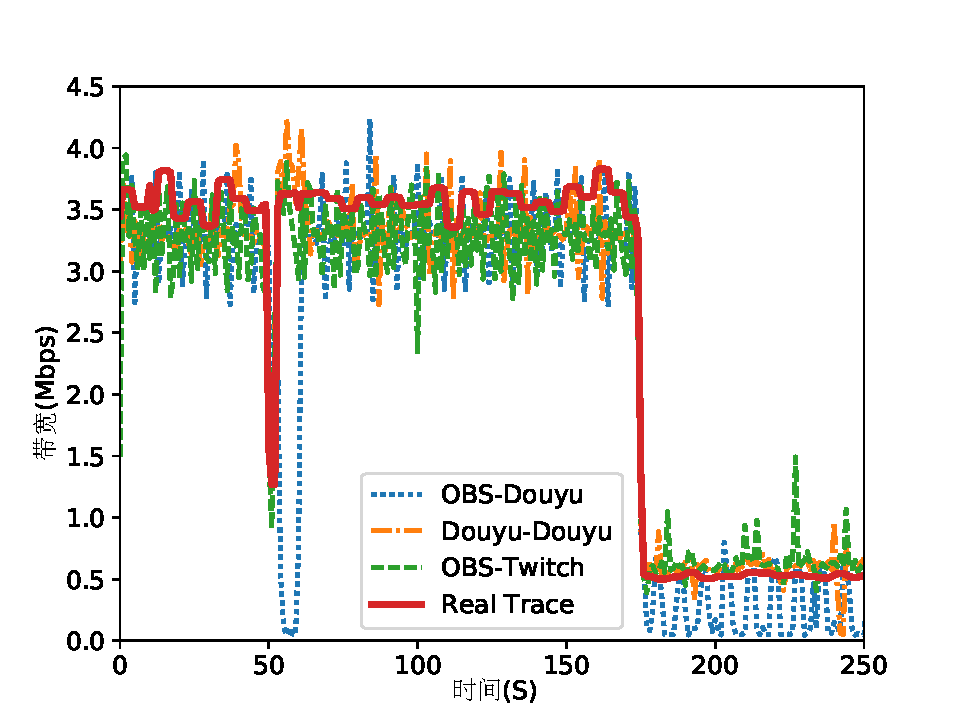
\includegraphics[width=0.7\textwidth]{vary-bandwidth}
  \caption{长时间带宽抖动状况下的吞吐量}
  \label{fig:vary-bandwidth}
\end{figure}

除了短时间带宽下降的测量实验之外,我们还验证了在长时间带宽下降的情况时商业平台的性能表现,如图~\ref{fig:vary-bandwidth}所示。与上面的实验配置大致相同,我们选取的初始码率3300kbps小于平均带宽,实验开始的一段时间里,实时的带宽一直高于初始的码率设置,主播端上传的视频播放很流畅。但在180秒之后时延带宽开始急剧的下降,降低到500kbps附近,实验期间我们一直持续观察码率变化,发现所有三组实验环境的码率始终保持不变,均维持在初始码率水平。但180秒之后,实时的码率大于可用带宽容量,视频数据产生的速度远远大于网络容量,观测到了大量的丢帧现象。OBS推流至斗鱼服务器的这组实验表现最差,甚至都没有充分利用带宽资源。尤其是180秒到250秒期间,这组实验的实时带宽在网络容量和零之间来回振荡。而观察其他两组实验,虽然整个过程中真实带宽紧跟网络容量变化,但180秒之后主播端一直在持续不断的丢帧。表~\ref{tb:drop}的后面三行记录了总共的丢帧数据,三组实验的上传失败百分比都很高,进一步说明了现有的商业平台处理长时间带宽下降的能力非常的有限。总的来说,现有的商业平台不能有效解决长时间带宽下降的情境下丢帧的问题。

\section{本质原因追溯}

\begin{figure}[htb]% use float package if you want it here
  \centering
  
\includegraphics[width=0.8\textwidth]{drop}
  \caption{视频帧队列示意图}
  \label{fig:drop}
\end{figure}

无论是有线网络环境还是无线网络环境,网络带宽抖动都时有发生。为了应对可能出现的带宽抖动,主播端应该会维护一个队列来存储等待发送的视频帧数据。主播端的视频帧队列的示意图如图~\ref{fig:drop}所示。主播端通过摄像头实时抓取画面,之后将抓取的画面送入编码器,编码成H264格式的视频帧;编码完成后的视频帧被编码器释放出来,进入视频帧队列排队等待被发送。同时发送数据的进程从队列中顺序取出一个视频帧,将它通过TCP蹭的socket端口发送到网络中去,整个视频编码发送的过程便是这样。如果网络状况不好,网络容量低于视频数据产生的速率,数据发送的进程会被堵塞住,视频帧队列累积到一定程度会超出最大空间容量的限制,之后新产生的视频帧直接被丢弃,不再纳入帧队列,于是发生了丢帧现象。另外,视频帧队列里的数据帧也会因为超出最大容量的限制,而有可能会丢弃。

\begin{figure}[h]
    \centering
%\small
    \begin{tabularx}{\linewidth}{rXXXXXXXXXXX}
        \toprule[1.5pt]
        帧类型       & I & B & B & P & B & B & P & B & B  & I  & ... \\ \midrule[1pt]
        播放顺序   & 1 & 2 & 3 & 4 & 5 & 6 & 7 & 8 & 9  & 10 & ... \\
        编码顺序 & 1 & 3 & 4 & 2 & 6 & 7 & 5 & 9 & 10 & 8  & ... \\
        \bottomrule[1.5pt]
    \end{tabularx}
    \caption{H.264帧的编码顺序和播放顺序}
    \label{fig:frame-order}
\end{figure}

丢帧现象产生的主要原因是网络堵塞。但大量的测量实验发现,丢帧可能还会在应用层造成放大效应。为了找到问题发生的根本原因,我们通过追溯开源直播软件OBS的源码,发现短时间的带宽抖动导致的丢帧放大效应主要是由于视频帧之间存在依赖关系。按照H264的编码标准,一段视频最后会被编码成一个图片组,称之为一个GoP(Group of Pictures)。编码协议规定,每个图片组的第一帧应保持原图不变,这一帧称为I帧,也称之为关键帧。P帧是利用前面已经编码的图像作为参考图像进行预测生成的,已经编码的图像包含前面的I帧和P帧;B帧则是一种双向预测,根据邻近的I帧和P帧产生。表~\ref{fig:frame-order}给出了一系列连续的视频帧的示意图,按照播放顺序展示。表中可以看出,视频帧的编解码的顺序和最后实际播放的顺序并不一定一致。考虑到一个GoP里视频帧之间的依赖关系,当一组GoP中间的P帧被丢弃的话,这个P帧之后所有的P帧和B帧都不能够正常解码。因此,如果网络带宽发生一次小抖动,导致一组GoP的中间或者开头出现丢帧现象,这个GoP剩余的帧都会被主播端丢弃,因此即使传输成功,也无法正常解码。这个原因导致我们在应用层观测到了放大效应,2秒的带宽抖动带来5-6秒的主播上传暂停。

\begin{algorithm}[htb]
\caption{OBS默认丢帧算法}
\label{alg:obs-drop}
{\bf Require:} timespan:队列时间长度;dropPFrame:和P帧相关的丢帧优先级;dropBFrame:和B帧相关的丢帧优先级;bandwidth:每个时隙的带宽
\begin{algorithmic}[1]
\State T1 := 0.9秒,T2:=0.7秒,timespan :=0
\If{新产生的帧是I帧}
\State dropPFrame := False, dropBFrame :=False
\State \Call{入队}{视频帧队列, 新产生的帧}
\State timespan:= timespan + 1
\EndIf
\If{新产生的帧是P帧}
\If{dropPFrame or timespan $>$ T1}
\State \Call{丢弃}{新产生的帧},丢弃所有的I帧和P帧
\State timespane := timespan - 丢弃的时长
\Else
\State \Call{入队}{视频帧队列, 新产生的帧}
\State timespan := timespan + 1
\EndIf
\EndIf
\If{新产生的帧是B帧}
\If{dropBFrame or timespan $>$ T2}
\State \Call{丢弃}{新产生的帧},丢弃所有的B帧
\State timespan := timespan - 丢弃的时长
\Else
\State \Call{入队}{视频帧队列,新产生的帧}
\State timespan := timespan + 1
\EndIf
\EndIf
\State timespan := timespan - \Call{发送的时长}{bandwidth}
\end{algorithmic}
\end{algorithm}


通过分析OBS主播软件的源码,我们破解了它的帧队列管理算法,如算法~\ref{alg:obs-drop}所示。OBS默认的丢帧算法引入了三个变量,P帧和B帧相关的丢帧优先级以及队列时间长度。丢帧优先级的设置是为了避免无效传输一些无法解码的视频帧,增加对网络带宽的利用率;队列时间长度表示队列中最旧的帧和当前时间刻度之间的差值。当主播端发生丢帧时,丢帧优先级被置为True,视频队列停止接收GoP中剩余的其他帧。一开始,所有的丢帧优先级都会被初始化为False。当一个新的视频帧产生时,先判断该帧是否是I帧,如果是,加入视频帧队列,并将所有的丢帧优先级赋值为False。因为I帧标志着一个新的GoP的开始,所以所有的丢帧优先级都被赋为初始值,同时,将队列的时间长度增加一个视频帧的时长。如果新产生的视频帧是P帧,判断队列时间长度是否小于0.9秒,以及P帧对应的丢帧优先级是否为True。如果队列时间长度大于0.9秒,或者P帧对应的丢帧优先级为True,则丢弃当前帧,B帧和P帧的丢帧优先级都被设为True。而且如果时间长度多余0.9秒,丢弃队列里所有的P帧和B帧,时间长度减去队列中丢弃帧的时间长度。上述两个条件均不满足的话,将新产生的P帧加入视频队列,和I帧操作相同。如果新产生的帧是B帧,队列时间长度的阈值变为0.7s,其余的逻辑和P帧类似。

大量的测量表明,当直播过程中发生带宽抖动的情况时,主播端的码率依然维持在初始的码率,视频数据产生的码率远远大于可用的无线带宽容量,便会发生丢帧现象。如果丢帧时丢弃了一个GoP中位置靠前的P帧,那么为了避免传输无效视频帧,该GoP剩余的其他视频帧都将会丢弃,映射到应用层面的表现为一段时间的上传暂停,我们称之为应用层的放大效应。通过对于开源直播软件的分析,我们可以确定地说问题发生的根本原因就是由于H264编码标准使得帧与帧之间存在依赖性。

\section{本章小结}
本章通过在实验室搭建的demo平台上的测量发现,开源的直播软件OBS目前并不能有效的应对移动网络的带宽抖动。当短时的带宽抖动发生时,在OBS平台上观测到短时的抖动会在应用层引起丢帧的放大效应;而当长时间带宽下降出现时,OBS直播平台并不能有效的应对,视频帧产生的速度一直保持不变,远远超于网络容量,造成长时间的上传视频质量不高。

为了验证在现行的商业平台上是否存在相同的问题,我们选取了OBS和斗鱼主播工具作为主播端,斗鱼服务器和Twitch服务器作为接收端,去重复我们上述的实验。在商业平台上的测量结果和demo平台的结果基本一致,表明目前的商业平台也尚未能有效地应对移动网络的带宽抖动。 通过解析OBS开源软件的源码,我们发现,应用层丢帧放大效应的主要原因是由于H264的编码标准导致帧与帧之间存在依赖性,长时间的带宽降低导致视频上传受到严重影响主要是由于视频的产生速率远远高于网络带宽容量。

为了解决上述问题,我们初步提出了两个方案,增加视频队列长度以及减少关键帧间隔。初步的仿真实验结果说明,两种方案都可以减少丢帧现象的发生,但是增加视频队列长度违反了帧传输及时性的要求。这为我们之后的优化空间提供了思路,视频队列长度应该严格控制在一个合理的阈值,将帧传输的时延控制在要求的范围内。